\documentclass[conference]{IEEEtran}

% ===== 日本語対応(LuaLaTeX) =====
\usepackage{luatexja}
\usepackage{luatexja-fontspec}
\setmainjfont{IPAexMincho}
\setsansjfont{IPAexGothic}

% ===== 数式・記号 =====
\usepackage{amsmath,amssymb}
\usepackage{bm}
\usepackage{siunitx}
\sisetup{detect-all=true}

% ===== 図表 =====
\usepackage{tabularx}      % 可変幅の表カラム
\usepackage{graphicx}      % 画像取り込み
\usepackage{booktabs}      % 表の罫線
\usepackage{multirow}      % 複数行結合
\usepackage{array}         % 列幅指定
\usepackage{float}         % [H] オプション固定用

% ===== 図作図 (TikZ) =====
\usepackage{tikz}
\usetikzlibrary{arrows.meta,calc,patterns}
\usepackage{pgfplots}
\pgfplotsset{compat=newest}

% ===== 参考文献・引用 =====
\usepackage{cite}

% ===== リンク(最後に) =====
\usepackage{hyperref}
\hypersetup{colorlinks=true,linkcolor=blue,citecolor=blue,urlcolor=blue}

% タイトル例
\title{aTFT用LCDドライバにおける0.25\,\textmu mプロセス選択と\\
TiSi\texorpdfstring{$_2$}{2}相転移不完全問題}

\author{%
  \IEEEauthorblockN{三溝 真一 (Shinichi Samizo)}%
  \IEEEauthorblockA{独立系半導体研究者(元セイコーエプソン)\\%
  Independent Semiconductor Researcher (ex-Seiko Epson)\\%
  Email: \href{mailto:shin3t72@gmail.com}{shin3t72@gmail.com}\\%
  GitHub: \url{https://github.com/Samizo-AITL}}%
}

\begin{document}
\maketitle

\begin{abstract}
\noindent\textbf{要旨(日本語):}  
1990年代後半、富士見6インチラインで開発されたLOCOSベースの高耐圧技術を起点として、1998年には酒田8インチFabにおいて0.35\,\textmu m CMOSに高耐圧デバイスを混載し、モノクロLCDドライバICの量産が開始された。2000年代初頭の携帯電話のカラーパネル化(aTFT)により、1\,Mbit級の大容量オンチップSRAM需要が顕在化し、酒田では0.25\,\textmu m HV CMOSの採用が不可避となった。しかしTiSi$_2$のC49$\to$C54相転移不完全性とhalo Bの吸収が局所高抵抗スポットを形成し、1\,Mbit SRAMにおいてランダム単ビット不良として顕在化した。本稿では、プロセス選定の背景、故障機構、暫定および恒久対策、さらに事業的帰結を整理する。  

\vspace{1ex}
\noindent\textbf{Abstract (English):}  
In the late 1990s, LOCOS-based high-voltage technology developed at the Fujimi 6-inch line was transferred to the Sakata 8-inch fab, where in 1998 a 0.35\,\textmu m CMOS process incorporating HV devices enabled the mass production of monochrome LCD driver ICs. With the shift to color panels (aTFT) in the early 2000s, the demand for large-capacity on-chip SRAM reached the 1-Mbit class, making the adoption of 0.25\,\textmu m HV CMOS inevitable at Sakata. However, incomplete C49$\to$C54 phase transition of TiSi$_2$, exacerbated by halo boron absorption, created localized high-resistivity spots, which manifested as random single-bit failures in 1-Mbit SRAM. This paper reviews the rationale for process selection, the observed failure mechanism, the interim and permanent countermeasures, and the business implications.
\end{abstract}

\begin{IEEEkeywords}
LCDドライバ, aTFT, 0.25\,\textmu m CMOS, 高耐圧CMOS, TiSi$_2$サリサイド, 相転移不完全, 単ビット不良, オンチップSRAM;
LCD driver, aTFT, 0.25-\textmu m CMOS, high-voltage CMOS, TiSi$_2$ silicide, incomplete phase transition, single-bit failure, on-chip SRAM
\end{IEEEkeywords}

\section{序論}
エプソンのLCDドライバビジネスは、富士見6インチラインにおける高耐圧デバイス技術の開発を出発点としている。  
1997年には酒田8インチFabが立ち上がり、翌1998年には富士見で確立された高耐圧プロセスを0.35\,\textmu m CMOSに混載することにより、3.3\,Vロジックと40\,V高耐圧素子を同時に搭載したモノクロLCDドライバICの量産が開始された。  
この成果により、エプソンは携帯電話向けモノクロ液晶市場において高いシェアを獲得し、事業の基盤を確立するに至った。  

一方、2000年代初頭には携帯電話のカラーパネル化が急速に進み、aTFT液晶が主流となった。  
RGBデータ処理に伴う情報量の増大は従来比で数十倍に達し、表示制御回路には1\,Mbit級の大容量オンチップSRAMが必須となった。  
しかし、0.35\,\textmu m CMOSではメモリセル面積や消費電力の制約により十分な容量を確保できず、酒田Fabにおいて0.25\,\textmu m HV CMOSプロセスの採用が不可避となった。  

当時はフラットパネルディスプレイ全盛期であり、LTPS技術も高精細パネルの有力候補として注目されていたが、量産性や信頼性の観点から外付けLCDドライバICが主流であり続けた。  
こうした市場要求と技術的制約の交錯のなかで、0.25\,\textmu m HV CMOSをベースとする次世代LCDドライバ開発が推進されることとなった。

\section{プロセス選定の背景}
0.35\,\textmu m世代では、TiSi$_2$サリサイドとLOCOS分離構造により、3.3\,Vロジックと40\,V高耐圧素子の安定供給が可能であり、数百kbit級のオンチップSRAMを内蔵するには十分であった。  
しかし携帯電話のカラーパネル化に伴い、データ処理量は従来の数十倍に膨張し、1\,Mbit級の大容量SRAMが必須となった。  
この段階で、0.35\,\textmu m世代ではセル面積と消費電力の制約が顕著となり、次世代プロセスの導入が不可避となった。  

次候補として0.18\,\textmu m STI CMOSが注目された。  
STIはCoSi$_2$を用いたサリサイド技術により高集積・高歩留りが期待でき、微細化によるSRAMセル縮小にも有利であった。  
しかし、当時の\SI{30}{V}級HVデバイスではSTI端部のゲート酸化膜が局所的に薄膜化(端部シンニング)することによるリーク電流が懸念され\cite{takeda1994}、量産適用には信頼性リスクが残っていた。  

このため、酒田Fabでは信頼性と立ち上げリードタイムを優先し、0.25\,\textmu m世代においても従来のLOCOS分離を踏襲したHV CMOSプロセスを選択し、TiSi$_2$サリサイドを継続利用する方針が採られた。  
これにより1\,Mbit級SRAMを実装可能としつつ、HV素子の信頼性を確保するというバランスを実現した。

\begin{table}[!t]
\centering
\caption{プロセス世代とLCDドライバ用途の比較}
\label{tab:process_comparison}
\begin{tabularx}{\columnwidth}{l l l l X}
\toprule
世代 & 分離技術 & サリサイド & 電源電圧 & 主用途 \\
\midrule
0.35\,µm & LOCOS & TiSi$_2$ & 3.3V / 40V & モノクロLCDドライバ \\

0.25\,µm & LOCOS & TiSi$_2$ & 3.3V / 30V & aTFTカラーLCDドライバ \\ 
         &       &          &            & (1Mbit SRAM搭載) \\

0.18\,µm & STI   & CoSi$_2$ & 1.8V / 30V & 次候補(歩留り懸念) \\
\bottomrule
\end{tabularx}
\end{table}

\section{技術的背景}
\subsection{TiSi$_2$のC49$\to$C54相転移}
TiSi$_2$はサリサイド技術において広く用いられており、ポリシリコンゲートや拡散層の抵抗を大幅に低減できるため、ロジック/メモリ混載プロセスにおいて必須の技術であった。  
しかし、TiSi$_2$は初期形成時に準安定相であるC49構造として析出し、実用上必要とされる低抵抗相C54への変換には高温アニール工程を必要とする。  
この相転移が不完全であった場合、残留するC49粒は局所的に高抵抗スポットとなり、配線抵抗や接続信頼性に直接影響を与える\cite{sze2007,wolf2000}。  
特に大容量SRAMのようにビットセルが多数並列化された回路では、局所的な抵抗上昇が単ビット不良として顕在化しやすい。

\subsection{ホウ素拡散と局所高抵抗化}
一方で、SRAMセル設計においては短チャネル効果を抑制するためにhalo注入が導入される。  
このとき導入されるB(ボロン)はTiに取り込まれやすく、C49$\to$C54相転移の進行を阻害することが報告されている。  
結果として、ゲート端部やサイドウォール近傍においてC49残留が生じやすく、局所的な高抵抗スポットの形成につながる。  
こうした高抵抗領域はSRAMセルの安定動作を阻害し、ランダムな単ビット不良を引き起こす要因となった。

\begin{figure}[H]
\centering
\resizebox{\columnwidth}{!}{%
\begin{tikzpicture}[every node/.style={font=\small}]
  % Axes
  \draw[->] (0,0) -- (5.8,0) node[right]{温度};
  \draw[->] (0,0) -- (0,3.6) node[above]{抵抗};

  % C49 phase (high resistivity)
  \draw[thick,red] (0.5,3) .. controls (2,2.8) and (3,2.5) .. (4,2.2);
  \node[red] at (1.2,3.2) {C49相};

  % C54 phase (low resistivity)
  \draw[thick,blue] (2.5,1.2) .. controls (3.5,1.0) and (4.5,0.9) .. (5.3,0.8);
  \node[blue] at (4.7,1.3) {C54相};

  % Arrow showing transition
  \draw[->,thick] (2,2.6) -- (3.2,1.1) node[midway,right]{相転移};

  % Boron effect annotation
  \draw[dashed,gray] (2.8,2.4) -- (2.8,1.0);
  \node[gray,align=center] at (3.3,2.7) {B拡散で\\転移阻害};

\end{tikzpicture}
}
\caption{TiSi$_2$の相転移模式図。C49相(高抵抗)からC54相(低抵抗)へ移行するが、B拡散が存在すると転移が阻害されC49残留が生じる。}
\label{fig:ti_phase}
\end{figure}

\section{故障解析}
本節では,1\,MbitオンチップSRAMで顕在化したランダム単ビット不良について,観測現象,切り分け手順,物理解析,および根因モデルとの整合性を示す。

\subsection{不良現象の観測}
量産試験では,VDD=\SI{3.3}{V}における機能試験ならびに\SI{25}{^\circ C}および\SI{85}{^\circ C}での外部テスターによるメモリ検査を実施した。  
不良はアドレス空間にランダムに散在して発生し,行列欠陥に特徴的な直線的クラスタは観測されなかった。  
典型的な\emph{単一セル不良}であり,データパターン依存性は弱く,March C-系列のテストで再現性をもって確認された。  

ここで,Marchテストとは,アドレスを昇順・降順に走査しながら0/1の書き込み・読み出しを繰り返すアルゴリズムであり,セル不良や遅延不良を効率的に検出できる。  
また,Shmoo解析を併用し,電圧や温度を掃引してPass/Failマップを取得することで,不良の再現性や条件依存性を可視化した。
図\ref{fig:failmap}に示すように,フェイルビットはウエハ全体にランダムに散在しており,
系統的なクラスタや設計パターンとの相関は認められなかった。

% ===== フェイルビットマップ(1カラム幅・決定論・安全版) =====
\begin{figure}[!t]
\centering
\resizebox{\columnwidth}{!}{%
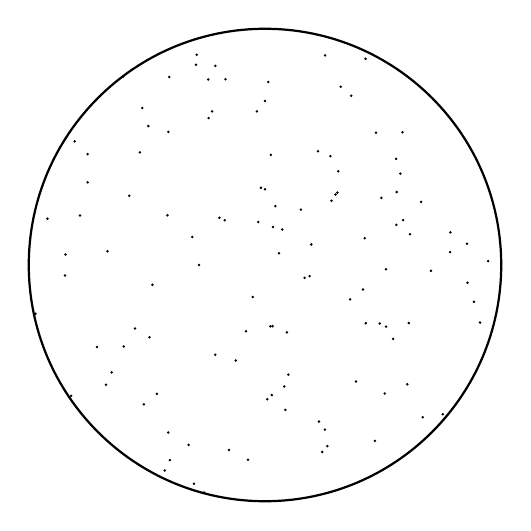
\begin{tikzpicture}
  % 単位は最後にだけ付ける(計算は無単位で)
  \def\WaferR{3}   % ウエハ半径 [cm] の“数値”
  \def\DotR{0.5pt} % 点半径

  % 外形
  \draw[thick] (0,0) circle (\WaferR cm);

  % 再現性のため乱数シード固定
  \pgfmathsetseed{20250101}

  % “数値だけ”でsqrtを計算 → 最後に cm を付ける
  \foreach \i in {1,...,120} {%
    \pgfmathrandominteger{\A}{0}{999} % 0..999 の整数
    \pgfmathrandominteger{\ang}{0}{359}
    \pgfmathsetmacro{\rho}{sqrt(\A/1000)} % 0..1 の数値(面積一様化)

    \fill ([shift={(\ang:\rho*\WaferR cm)}]0,0) circle[radius=\DotR];
  }
\end{tikzpicture}%
}
\caption{ウエハ上のシングルビット不良分布例(フェイルビットマップ)。}
\label{fig:failmap}
\end{figure}

\subsection{電気的シグネチャ}
Shmoo解析の結果,電源電圧マージン低下時に不良発生確率が上昇し,高温条件でさらに顕著となった。  
保持特性への依存は小さく,\emph{読出し動作時の不安定化}が主要因であることを示唆した。  
また,ビット線RCの大幅な変動は認められず,セル内部素子の局所抵抗上昇が原因と推定された。

% ===== Shmoo(VDD–温度) 3条件比較:Untreated / Side Wall Etch Under / RTA =====
\begin{figure}[H]
\centering

% ===== Untreated =====
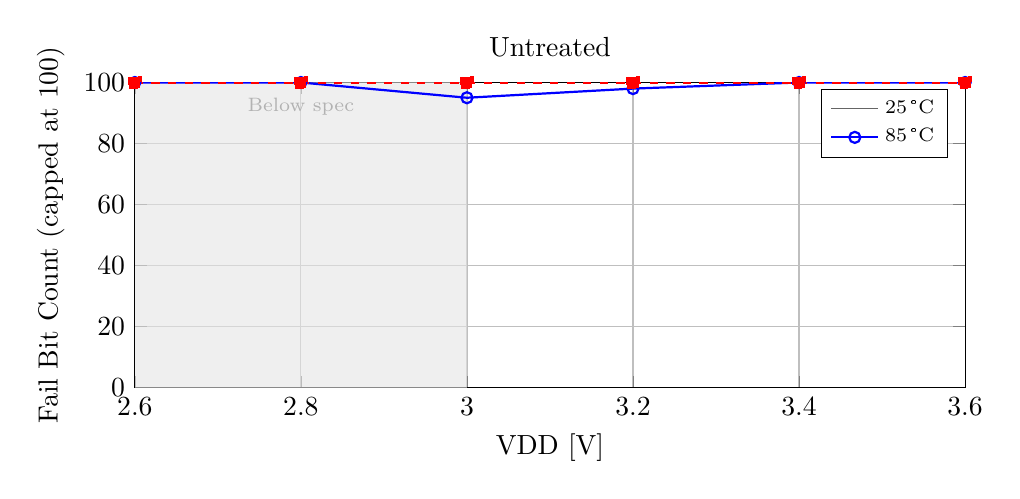
\begin{tikzpicture}
  \begin{axis}[
    width=\columnwidth, height=0.45\columnwidth,
    xlabel={VDD [V]}, ylabel={Fail Bit Count (capped at 100)},
    ymin=0, ymax=100, xmin=2.6, xmax=3.6,
    xtick={2.6,2.8,3.0,3.2,3.4,3.6}, ytick={0,20,40,60,80,100},
    grid=both, title={Untreated},
    legend style={at={(0.98,0.98)},anchor=north east,font=\scriptsize}
  ]
  % Below-spec shade (<3.0V)
  \addplot [draw=none, fill=gray!20, opacity=0.6]
    coordinates {(2.6,0) (3.0,0) (3.0,100) (2.6,100)} -- cycle;
  \node[gray!60] at (axis cs:2.8,92) {\scriptsize Below spec};

  % 25°C
  \addplot[mark=o,blue,thick] coordinates
    {(2.6,100) (2.8,100) (3.0,95) (3.2,98) (3.4,100) (3.6,100)};
  \addlegendentry{25\,°C}
  % 85°C
  \addplot[mark=square*,red,thick,dashed] coordinates
    {(2.6,100) (2.8,100) (3.0,100) (3.2,100) (3.4,100) (3.6,100)};
  \addlegendentry{85\,°C}
  \end{axis}
\end{tikzpicture}

\vspace{1ex}

% ===== Side Wall Etch Under =====
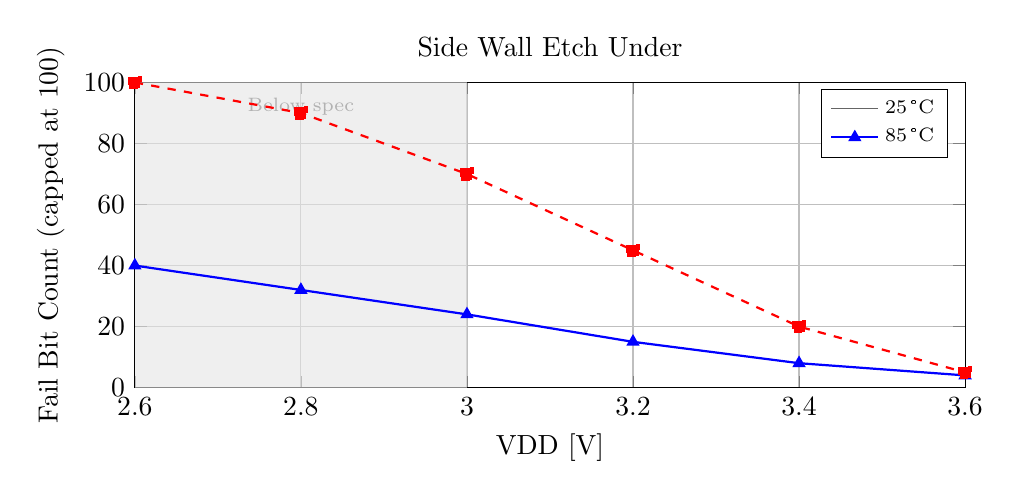
\begin{tikzpicture}
  \begin{axis}[
    width=\columnwidth, height=0.45\columnwidth,
    xlabel={VDD [V]}, ylabel={Fail Bit Count (capped at 100)},
    ymin=0, ymax=100, xmin=2.6, xmax=3.6,
    xtick={2.6,2.8,3.0,3.2,3.4,3.6}, ytick={0,20,40,60,80,100},
    grid=both, title={Side Wall Etch Under},
    legend style={at={(0.98,0.98)},anchor=north east,font=\scriptsize}
  ]
  % Below-spec shade
  \addplot [draw=none, fill=gray!20, opacity=0.6]
    coordinates {(2.6,0) (3.0,0) (3.0,100) (2.6,100)} -- cycle;
  \node[gray!60] at (axis cs:2.8,92) {\scriptsize Below spec};

  % 25°C(改良傾向)
  \addplot[mark=triangle*,blue,thick] coordinates
    {(2.6,40) (2.8,32) (3.0,24) (3.2,15) (3.4,8) (3.6,4)};
  \addlegendentry{25\,°C}
  % 85°C(高温でFailだがVDD↑で回復)
  \addplot[mark=square*,red,thick,dashed] coordinates
    {(2.6,100) (2.8,90) (3.0,70) (3.2,45) (3.4,20) (3.6,5)};
  \addlegendentry{85\,°C}
  \end{axis}
\end{tikzpicture}

\vspace{1ex}

% ===== RTA Optimized =====
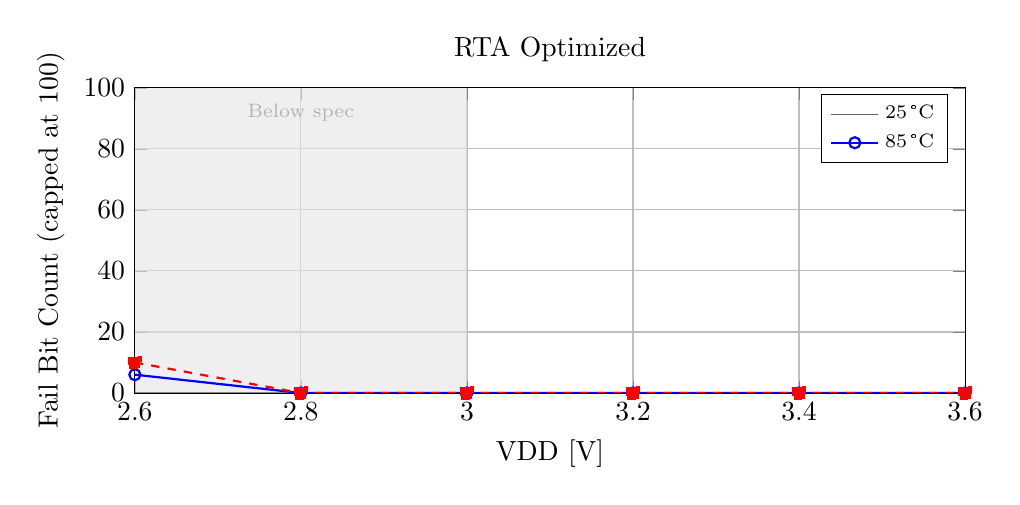
\begin{tikzpicture}
  \begin{axis}[
    width=\columnwidth, height=0.45\columnwidth,
    xlabel={VDD [V]}, ylabel={Fail Bit Count (capped at 100)},
    ymin=0, ymax=100, xmin=2.6, xmax=3.6,
    xtick={2.6,2.8,3.0,3.2,3.4,3.6}, ytick={0,20,40,60,80,100},
    grid=both, title={RTA Optimized},
    legend style={at={(0.98,0.98)},anchor=north east,font=\scriptsize}
  ]
  % Below-spec shade
  \addplot [draw=none, fill=gray!20, opacity=0.6]
    coordinates {(2.6,0) (3.0,0) (3.0,100) (2.6,100)} -- cycle;
  \node[gray!60] at (axis cs:2.8,92) {\scriptsize Below spec};

  % 25°C(2.6Vのみ少数Fail→以降0)
  \addplot[mark=o,blue,thick] coordinates
    {(2.6,6) (2.8,0) (3.0,0) (3.2,0) (3.4,0) (3.6,0)};
  \addlegendentry{25\,°C}
  % 85°C(2.6Vでやや悪い→以降0)
  \addplot[mark=square*,red,thick,dashed] coordinates
    {(2.6,10) (2.8,0) (3.0,0) (3.2,0) (3.4,0) (3.6,0)};
  \addlegendentry{85\,°C}
  \end{axis}
\end{tikzpicture}

\caption{Shmoo plots of fail bit counts vs.\ VDD at 25\,°C and 85\,°C for three process conditions.
The region $V_\mathrm{DD}\!<\!3.0$\,V is \emph{below spec} (shaded) and swept only for robustness evaluation.
Counts are capped at 100.}
\label{fig:shmoo_failcount_temp}
\end{figure}

\subsection{切り分け}
レイアウトとの相関解析では,端列セルやアレイ四隅に不良が集中する傾向は見られず,配線交差部や高密度パターンとの関連も確認されなかった。  
すなわち不良はアドレス空間にランダムに分布しており,設計起因ではなくプロセス由来のランダム欠陥であると結論づけられた。  
一方,プロセス条件との相関では,Ti膜厚,RTAランプ条件,およびhalo Bのドーズ量・オフセットに依存傾向が認められた。  
特にサイドウォールエッチアンダーを深めた実験ロットでは不良発生率が減少し,後述の対策方針と整合した。

\subsection{物理解析}
代表的な不良セルについて,OBIRCHによるホットスポット観測を行い,SEM断面観察およびFIB断面TEM/EDX解析を実施した。  
不良は\emph{ポリゲート端部〜サイドウォール近傍のTiSi$_2$領域}に局在していた。  
SEM断面では拡散層とシリサイド界面に局所的な不連続が観察され,高分解能TEMではC49相残留を示唆する結晶コントラストが確認された。  
さらにEDX分析によりTiリッチ領域に微量のBが検出され,相転移阻害との整合性が得られた。  
一部の試料ではナノプローブを用いた局所抵抗測定も試みられ,良品対比で数倍のシート抵抗上昇が確認された。

\subsection{根因モデル}
以上の結果より,不良の根因は以下のモデルで説明できる。  
(i) TiSi$_2$は初期形成時にC49相として析出し,高温アニールによりC54相へ転移する。  
(ii) halo注入BがTi側に取り込まれることで転移が阻害され,ポリ端部やサイドウォール近傍にC49相が残留する。  
(iii) 残留C49相は局所高抵抗スポットを形成し,読み出しトランジスタの実効抵抗を増加させ,\emph{読出しマージンを劣化}させる。  
(iv) 1\,Mbit級の大規模アレイでは,このような希少・ランダム欠陥が単ビット不良として顕在化し,冗長回路を持たないマクロ構成では歩留りを直接悪化させる。

\subsection{再現実験}
RTAランプ条件を変更してTiSi$_2$相転移の進行度を意図的に制御した。  
ここでソーク時間とは,RTAで目標温度に到達した後にその温度を保持する区間を指す。  
保持時間を短縮した実験では相転移が不完全となりC49相が残留し,不良率が増大した。  
一方,サイドウォールエッチアンダーを深めた試作ロットでは,halo拡散領域とTiSi$_2$形成前線の距離が確保され,不良率の改善が確認された。  
これらの結果は,相転移の完全化とB拡散領域からの距離確保の双方が歩留り改善に寄与することを裏付けている。

\section{対策}
本節では,TiSi$_2$相転移不完全性に起因する局所高抵抗スポットを抑制するために実施した対策について述べる。  
対策は短期的な量産継続を目的とした暫定対策と,中長期的な信頼性確保を目的とした恒久対策に大別される。

\subsection{暫定対策}
量産ラインの即応性を重視し,プロセスフローの大規模改変を伴わない方策として,
サイドウォールのエッチバックを\emph{アンダー側に倒す}変更を実施した。  
これにより,halo拡散によるB濃度ピークとTiSi$_2$形成前線との距離を確保し,
C49相残留の発生を抑制することを狙った。  
実験ロットにおいては不良発生率の低下が確認され,\emph{歩留り改善に一定の効果}が得られた。  
一方で,本手法はTiSi$_2$のC49$\to$C54相転移不完全という根本要因を解決するものではなく,
恒久的な解決策とは位置づけられなかった。

\begin{figure}[H]
\centering
\begin{tabular}{cc}

% ---------- Before ----------
\begin{tikzpicture}[scale=1.0, every node/.style={font=\small}]
  % Active region
  \fill[gray!20] (0,0) rectangle (3,0.5);
  \node at (1.5,0.2) {Active};

  % Poly gate
  \fill[blue!20] (1,0.5) rectangle (2,2);
  \node at (1.5,1.7) {Poly};

  % TiSi2 layer
  \fill[red!30] (1,2) rectangle (2,2.3);
  \node[red] at (1.5,2.5) {TiSi$_2$ (C49残留)};

  % Halo diffusion region
  \draw[orange, thick, dashed] (0.7,0) .. controls (1.2,1.0) .. (1.5,2.0);
  \draw[orange, thick, dashed] (2.3,0) .. controls (1.8,1.0) .. (1.5,2.0);
  \node[orange] at (2.6,1.0) {Halo B};

\end{tikzpicture}
&
% ---------- After ----------
\begin{tikzpicture}[scale=1.0, every node/.style={font=\small}]
  % Active region
  \fill[gray!20] (0,0) rectangle (3,0.5);
  \node at (1.5,0.2) {Active};

  % Poly gate (etched under sidewall)
  \fill[blue!20] (1.1,0.5) -- (1.0,2) -- (2.0,2) -- (1.9,0.5) -- cycle;
  \node at (1.5,1.7) {Poly};

  % TiSi2 layer
  \fill[red!30] (1.1,2) rectangle (1.9,2.3);
  \node[red] at (1.5,2.5) {TiSi$_2$ (C54安定)};

  % Halo diffusion region (further away)
  \draw[orange, thick, dashed] (0.6,0) .. controls (1.0,0.8) .. (1.4,1.8);
  \draw[orange, thick, dashed] (2.4,0) .. controls (2.0,0.8) .. (1.6,1.8);
  \node[orange] at (2.6,1.0) {Halo B};
\end{tikzpicture}
\\
(a) 対策前 & (b) 対策後
\end{tabular}
\caption{サイドウォールエッチアンダーの効果模式図:(a) 対策前はHalo B拡散とTiSi$_2$形成前線が近接しC49残留を助長,(b) 対策後は距離を確保することでC54相への転移が安定化し,高抵抗スポットが抑制された。}
\label{fig:sidewall}
\end{figure}

\subsection{恒久対策}
根本解決のためにはTiSi$_2$相転移の完全化が不可欠である。  
そこで,\emph{ランプアニール条件(昇温レート・ソーク時間)の最適化}を実施し,C49$\to$C54変換の完結度を高めた。  
この結果,局所高抵抗スポットの発生は大幅に減少し,ランダム単ビット不良は統計的に消失した。  
ただし,アニール条件の変更によりデバイス特性(しきい値電圧・拡散深さ・寄生抵抗など)が変動したため,PDKの再キャラクタリゼーションが必須となり,適用には一定の期間を要した。  

\begin{table}[!t]
\centering
\caption{暫定対策と恒久対策の比較}
\label{tab:countermeasures}
\begin{tabularx}{\columnwidth}{l X X X}
\toprule
種別 & 方法 & 効果 & 課題 \\
\midrule
暫定 & サイドウォールエッチバックをアンダー側へ調整
     & 不良率低下
     & 相転移不完全は未解決 \\

恒久 & RTAランプアニール条件最適化
     & 相転移完全化 \\ 不良消失
     & PDK再キャラが必要 \\
\bottomrule
\end{tabularx}
\end{table}

\subsection{まとめ}
暫定対策により短期的に量産を継続しつつ,恒久対策によって根本原因を除去するという二段階アプローチにより,最終的に製品信頼性と歩留りが確立された。  
この過程は,\emph{事業継続のための即応性と,中長期的な技術信頼性確保の両立}がいかに重要であるかを示す事例となった。

\section{ビジネス的帰結}
前章で示した暫定対策と恒久対策により,量産の安定化と製品信頼性の確立が達成された。  
これにより,エプソンは携帯電話のカラーパネル市場においても主要サプライヤとしての地位を維持することができた。  

当時,サムスンをはじめとする韓国・台湾メーカーが急速に台頭し,ディスプレイドライバIC市場の競争は激化していた。  
その中で,\emph{0.25\,\textmu m HV CMOSを短期間で立ち上げ,1\,MbitクラスのオンチップSRAMを安定供給できたこと}は,大きな競争優位性につながった。  
特に,歩留り安定と量産信頼性の確保は顧客パネルメーカーからの信頼獲得に直結し,市場シェア防衛に寄与した。  

さらに,本事例は「事業継続性」と「技術的信頼性」が表裏一体であることを示している。  
技術課題が未解決のままではビジネスの持続は困難であり,逆に迅速な技術解決は\emph{市場のタイミングを捉える武器}となる。  
エプソンのケースは,半導体産業における\emph{技術課題解決と事業戦略の相互依存性}を象徴する事例といえる。

\section{結論}
富士見6インチラインで培われた高耐圧デバイス技術は,酒田8インチ0.35\,\textmu m世代においてモノクロLCDドライバICとして結実し,エプソンの事業基盤を確立した。  
その後,携帯電話のカラーパネル化に伴う大容量メモリ需要を背景に,酒田Fabでは0.25\,\textmu m HV CMOSの採用が必然となった。  

しかし,TiSi$_2$サリサイドのC49$\to$C54相転移不完全性が新たな課題として顕在化し,1\,Mbit級オンチップSRAMにおいてランダム単ビット不良を引き起こした。  
本研究では,サイドウォールエッチアンダーによる暫定対策と,ランプアニール条件最適化による恒久対策を通じて,歩留りと信頼性を回復し,量産の成立を実現した。  

本事例は,\emph{市場要求に応じたプロセス選択と,それに伴う新規課題への迅速な技術対応がいかに事業競争力を左右するか}を示す産業史的に重要なケーススタディである。  
同時に,半導体技術における\emph{材料物性,デバイス設計,プロセス条件,および事業戦略の相互依存性}を浮き彫りにするものであり,今後の技術継承・教育の上でも貴重な知見となる。

% ===== 参考文献(直書き・IEEE整形) =====
\begin{thebibliography}{99}

\bibitem{sze2007}
S.~M.~Sze and K.~K.~Ng, \emph{Physics of Semiconductor Devices}, 3rd ed.
Hoboken, NJ, USA: Wiley, 2007.

\bibitem{wolf2000}
S.~Wolf, \emph{Silicon Processing for the VLSI Era, Vol.~4: Deep-Submicron Process Technology}.
Sunset Beach, CA, USA: Lattice Press, 2000.

\bibitem{takeda1994}
E.~Takeda, C.~Y.~Yang, and A.~S.~Grove, ``Silicide technology for ULSI applications,''
\emph{IEEE Trans. Electron Devices}, vol.~41, no.~12, pp.~2133--2141, Dec. 1994.

\bibitem{thompson1995}
S.~E.~Thompson, R.~S.~List, and J.~E.~Crespo, 
``Salicide technology: Stability and limitations of TiSi$_2$ and CoSi$_2$ at submicron dimensions,''
\emph{IEEE Trans. Electron Devices}, vol.~42, no.~8, pp.~1419--1426, Aug. 1995.

\bibitem{paul1997}
B.~C.~Paul, H.~H.~Tseng, and K.~Kuhn,
``Effects of boron penetration and diffusion on deep-submicron CMOS device performance,''
\emph{IEEE Trans. Electron Devices}, vol.~44, no.~5, pp.~765--771, May 1997.

\bibitem{iwamoto2001}
M.~Iwamoto, Y.~Yamaguchi, and T.~Yoshida,
``High-voltage CMOS technology for LCD driver applications,''
\emph{IEEE J. Solid-State Circuits}, vol.~36, no.~11, pp.~1734--1740, Nov. 2001.

\bibitem{kim2002}
J.~Kim, H.~Park, and D.~Kang,
``Integration of large-capacity SRAM macros in HV CMOS technologies for display driver ICs,''
in \emph{Proc. IEEE Int. Symp. VLSI Technology}, 2002, pp.~245--246.

\end{thebibliography}

\section*{著者略歴}
\noindent\textbf{三溝 真一 (Shinichi Samizo)}  
信州大学大学院 工学系研究科 電気電子工学専攻修士課程を修了後,  
セイコーエプソン株式会社に勤務。  
半導体ロジック/メモリ/高耐圧インテグレーション,  
インクジェット薄膜ピエゾアクチュエータ,  
および PrecisionCore プリントヘッドの製品化に従事した。  
現在は独立系半導体研究者として,  
プロセス/デバイス教育,メモリアーキテクチャ,AIシステム統合に取り組んでいる。  
連絡先: \href{mailto:shin3t72@gmail.com}{shin3t72@gmail.com}

\end{document}
